\documentclass[11pt,a4paper,oldfontcommands,oneside]{memoir}
\usepackage[utf8]{inputenc}
\usepackage{microtype}
\usepackage[dvips]{graphicx}
\usepackage{xcolor}
\usepackage{times}
\usepackage{graphicx}
\usepackage[spanish]{babel}
\usepackage[
breaklinks=true,colorlinks=true,
%linkcolor=blue,urlcolor=blue,citecolor=blue,% PDF VIEW
linkcolor=black,urlcolor=black,citecolor=black,% PRINT
bookmarks=true,bookmarksopenlevel=2]{hyperref}

\usepackage{geometry}
% PDF VIEW
% \geometry{total={210mm,297mm},
% left=25mm,right=25mm,%
% bindingoffset=0mm, top=25mm,bottom=25mm}
% PRINT
\geometry{total={210mm,297mm},
left=20mm,right=20mm,
bindingoffset=10mm, top=25mm,bottom=25mm}

\OnehalfSpacing
%\linespread{1.3}

%%% CHAPTER'S STYLE
\chapterstyle{bianchi}
%\chapterstyle{ger}
%\chapterstyle{madsen}
%\chapterstyle{ell}
%%% STYLE OF SECTIONS, SUBSECTIONS, AND SUBSUBSECTIONS
\setsecheadstyle{\Large\bfseries\sffamily\raggedright}
\setsubsecheadstyle{\large\bfseries\sffamily\raggedright}
\setsubsubsecheadstyle{\bfseries\sffamily\raggedright}


%%% STYLE OF PAGES NUMBERING
%\pagestyle{companion}\nouppercaseheads 
%\pagestyle{headings}
%\pagestyle{Ruled}
\pagestyle{plain}
\makepagestyle{plain}
\makeevenfoot{plain}{\thepage}{}{}
\makeoddfoot{plain}{}{}{\thepage}
\makeevenhead{plain}{}{}{}
\makeoddhead{plain}{}{}{}


\maxsecnumdepth{subsection} % chapters, sections, and subsections are numbered
\maxtocdepth{subsection} % chapters, sections, and subsections are in the Table of Contents


%%%---%%%---%%%---%%%---%%%---%%%---%%%---%%%---%%%---%%%---%%%---%%%---%%%

\begin{document}

%%%---%%%---%%%---%%%---%%%---%%%---%%%---%%%---%%%---%%%---%%%---%%%---%%%
%   TITLEPAGE
%
%   due to variety of titlepage schemes it is probably better to make titlepage manually
%
%%%---%%%---%%%---%%%---%%%---%%%---%%%---%%%---%%%---%%%---%%%---%%%---%%%
\thispagestyle{empty}

{%%%
\sffamily
\centering
\Large

~\vspace{\fill}

\includegraphics[scale=0.5]{marcos.png} \\
{\huge 
\vspace{2cm}
3.2 Importación CAD a Gazebo
}
\vspace{2.5cm}

{\LARGE
César Omar Alvarado Contreras \\
Jonathan Fonseca Camarena \\
Marcos Manzo Torres \\
Eduardo Robles Vázquez \\
Víctor Gabriel Tapia Casillas

}

\vspace{2.5cm}

Universidad Politécnica de la Zona Metropolitana de Guadalajara

\vspace{3.5cm}

Profesor: Carlos Enrique Morán Garabito

\vspace{\fill}

8 de noviembree del 2019

%%%
}%%%

\vspace{.5cm}
\hfill\break




\tableofcontents*

\clearpage

%%%---%%%---%%%---%%%---%%%---%%%---%%%---%%%---%%%---%%%---%%%---%%%---%%%
%%%---%%%---%%%---%%%---%%%---%%%---%%%---%%%---%%%---%%%---%%%---%%%---%%%
\chapter{Blender}
Blender es un programa informático multi plataforma, dedicado especialmente al modelado, iluminación, renderizado, animación y creación de gráficos tridimensionales. También de composición digital utilizando la técnica procesal de nodos, edición de vídeo, escultura (incluye topología dinámica) y pintura digital.\\ 

El programa fue inicialmente distribuido de forma gratuita pero sin el código fuente, con un manual disponible para la venta, aunque posteriormente pasó a ser software libre. Actualmente es compatible con todas las versiones de Windows, macOS, GNU/Linux (incluyendo Android), Solaris, FreeBSD e IRIX. \\

\begin{figure}
\begin{center}
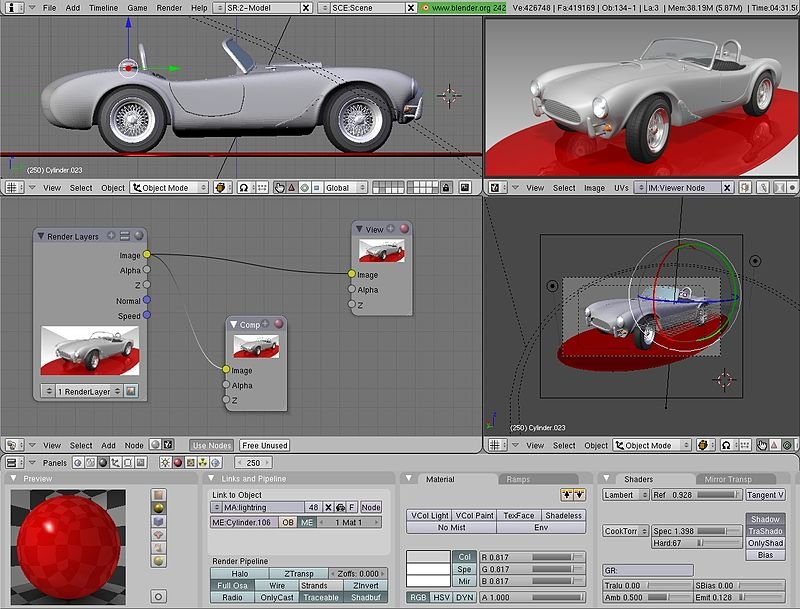
\includegraphics[scale=.4]{blender.jpg}
\end{center}
\caption{Ejemplo de las capacidades de Blender.}
\label{blender}:
\end{figure}

\chapter{Gazebo}

Gazebo es un simulador de robótica en 3D de código abierto. Gazebo integró el motor físico ODE de renderizado de OpenGL y código de soporte para la simulación y control de actuadores. En 2011, Gazebo se convirtió en un proyecto independiente apoyado por Willow Garage.\\
En 2012, la Fundación de robótica de código abierto (OSRF por sus siglas en inglés)se convirtio en el administrador del proyecto Gazebo. Posteriormente, la OSRF cambió su nombre a Open Robotics en 2018. \\ 
Gazebo puede utilizar multiples motores físicos de alto desempeño, como ODE, Bullet, etc (Por defecto viene siendo ODE). Este provee de renderizados realistas de ambientes, incluyendo iluminaciones, sombras y texturas, todas estas de gran calidad. Puede modelar senosres que pueden "ver" el ambiente simulado, como buscadores láser de rango, cámaras y sensores del estilo Kinect entre otros.

\begin{figure}
\begin{center}
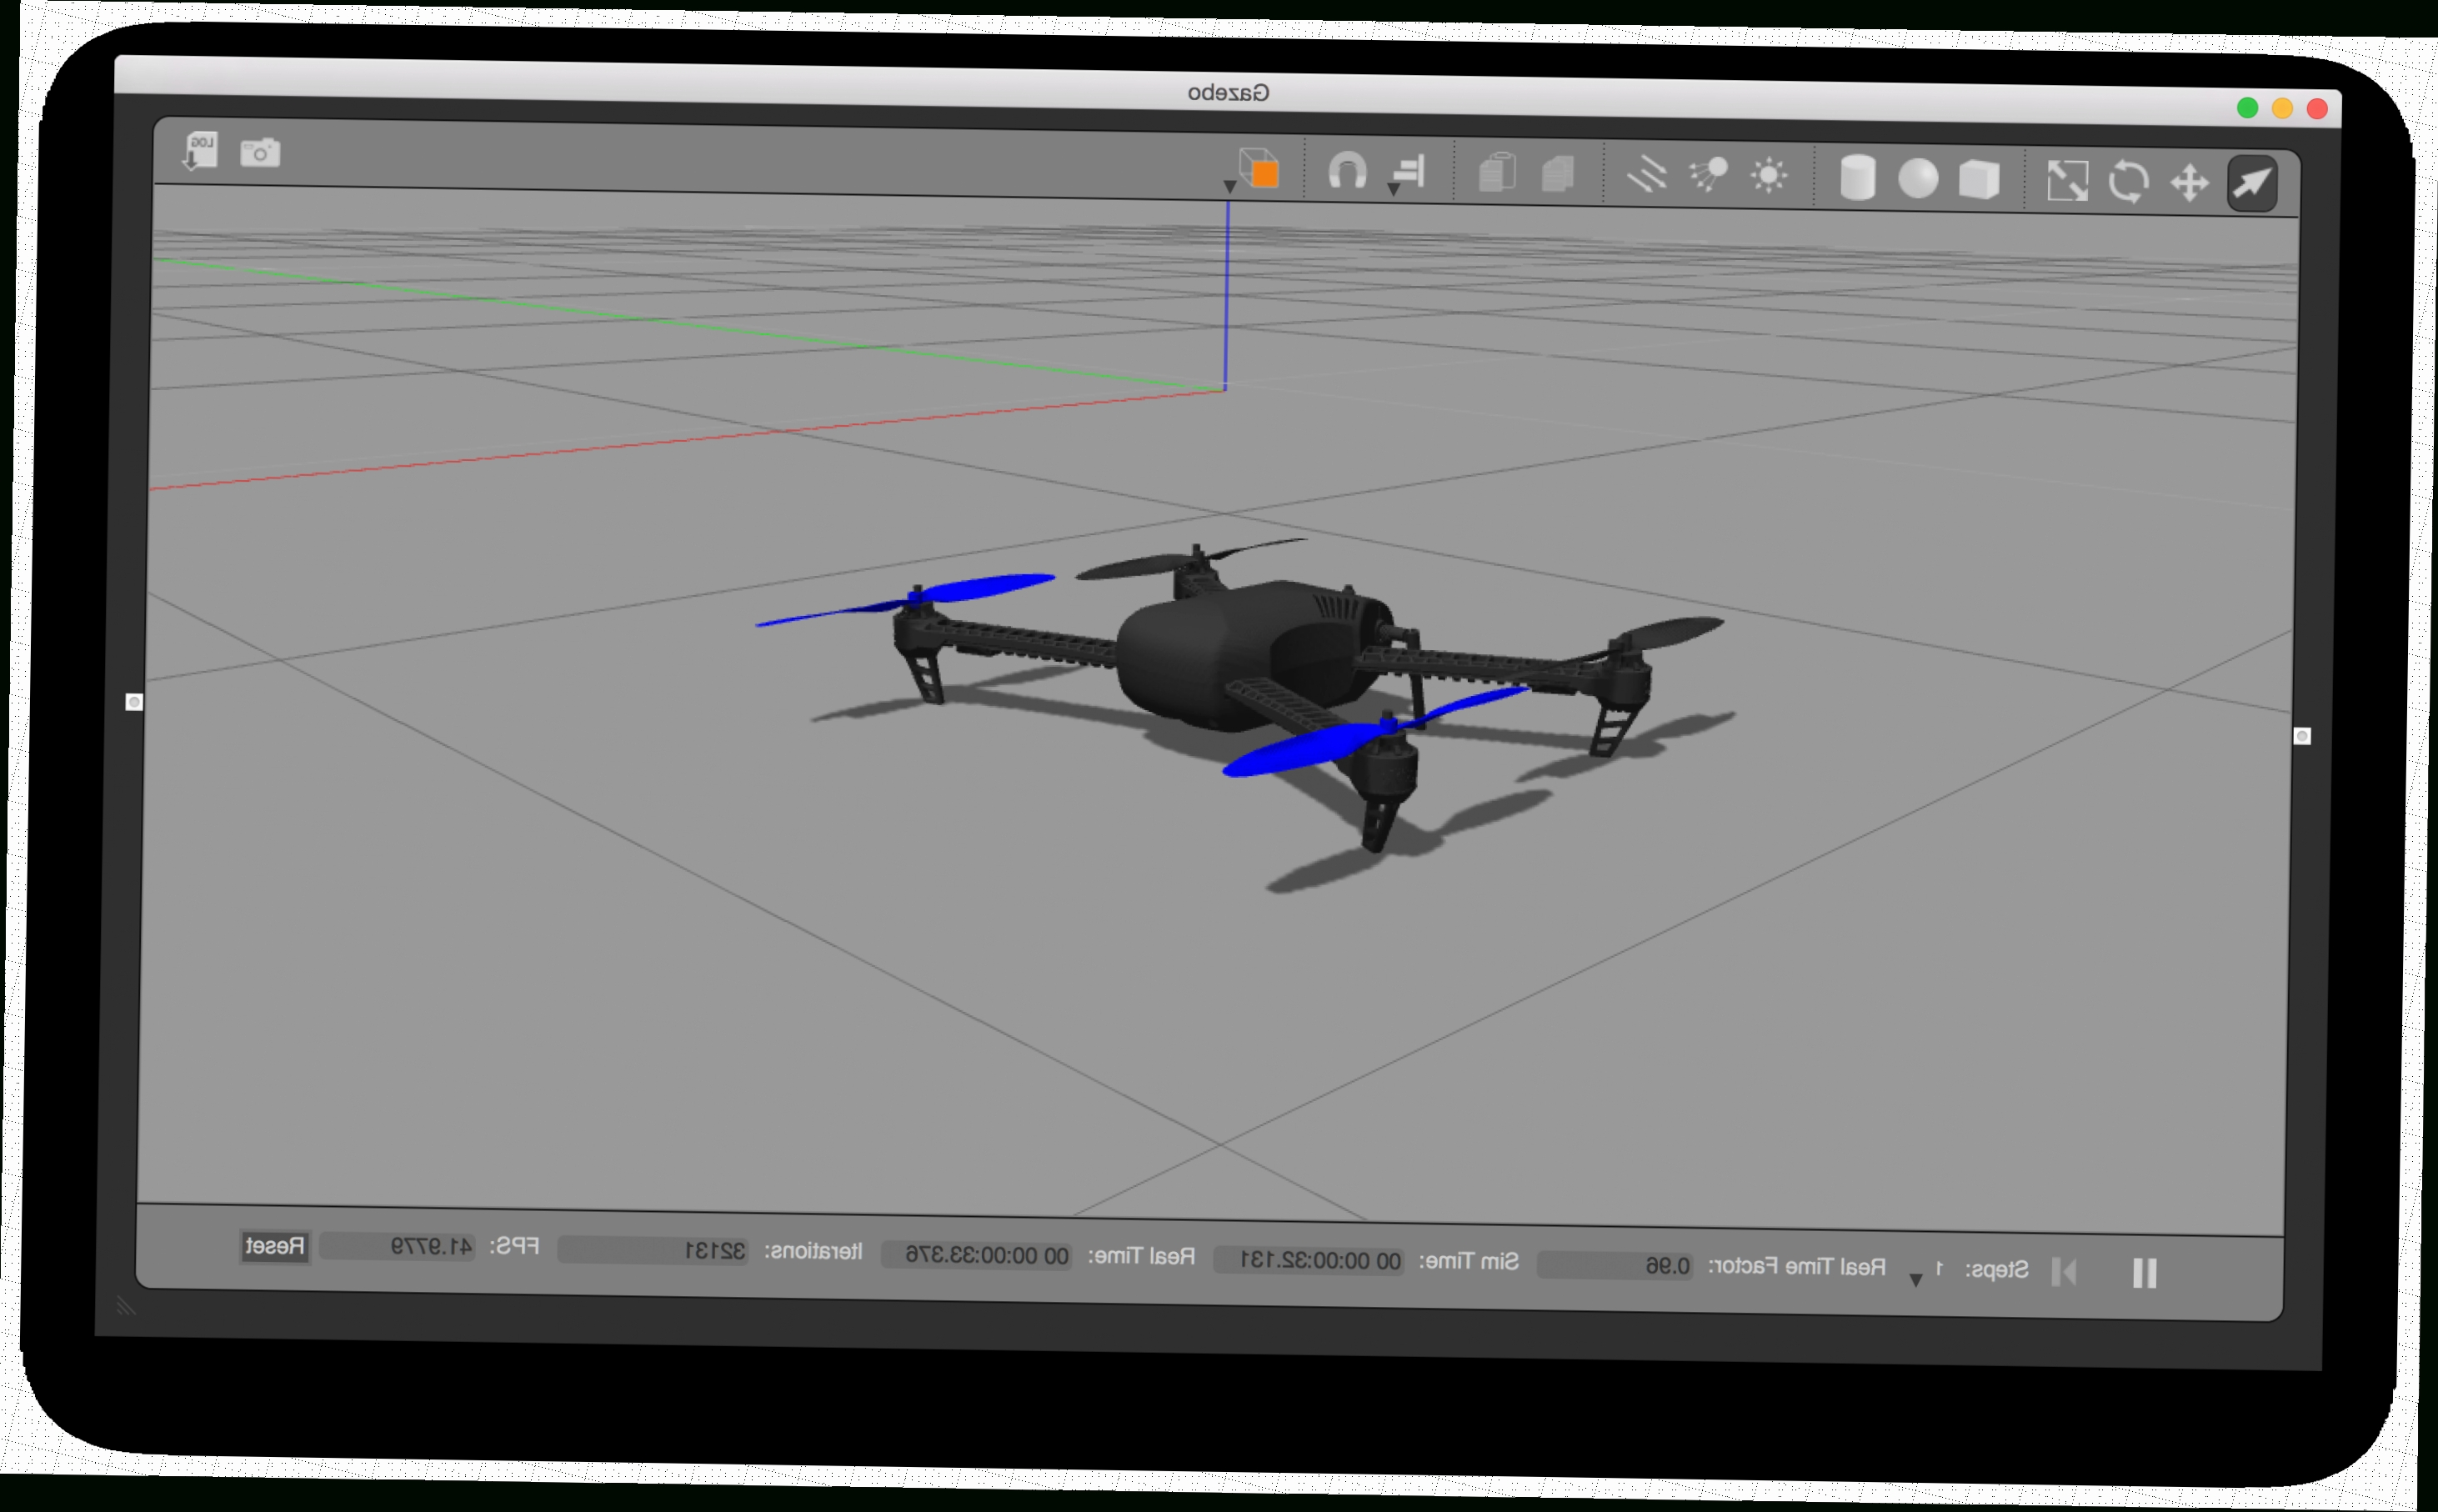
\includegraphics[scale=.12]{gazebo.jpg}
\end{center}
\caption{Ejemplo de las capacidades de Gazebo.}
\label{blender}:
\end{figure}


\chapter{Desarrollo}
Primeramente y partiendo del ensamble realizado en SolidWorks, exportamos dicho ensamble como .STL con lo cual el archivo podrá importarse en Blender de manera sencilla por medio de mallas.

\begin{figure}[h]
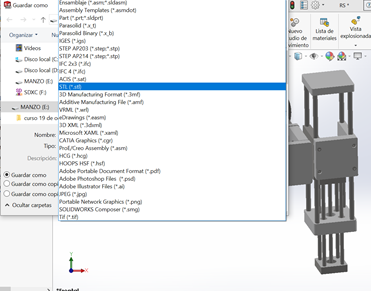
\includegraphics[scale=.9]{1.png}
\caption{Exportación en SolidWorks}
\label{Imagen 1}
\end{figure}
Iniciamos nuestra máquina virtual, donde trabajaremos con el archivo .STL
\begin{figure}[h]
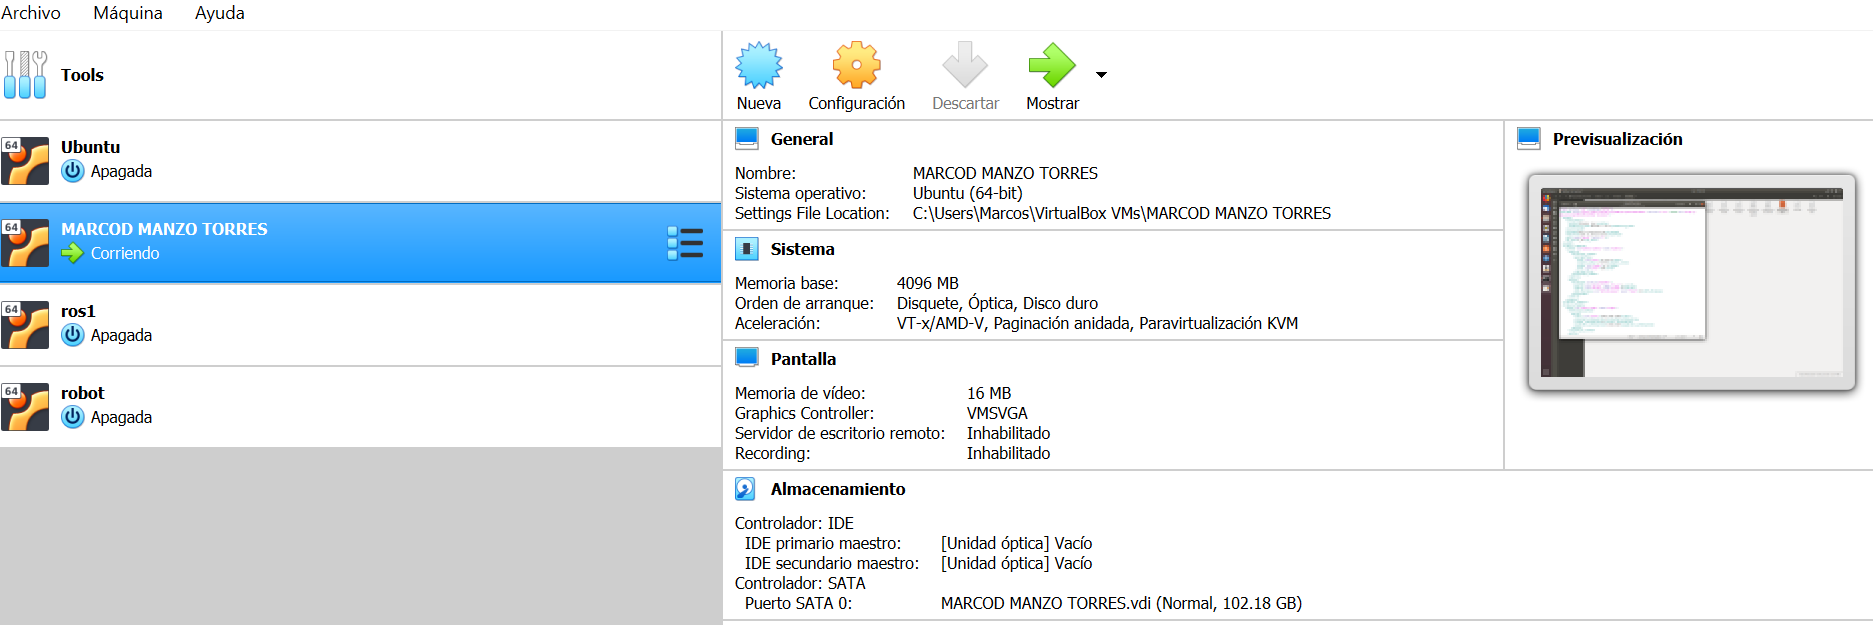
\includegraphics[scale=.7]{maquina.png}
\caption{Inicio de máquina virtual}
\label{Imagen 2}
\end{figure}\\
Abrimos una terminal en nuestro sistema Ubuntu, y colocamos el nombre de blender para abrir el programa y comenzar a trabajar.

\begin{figure}[h]
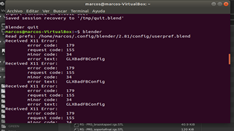
\includegraphics[scale=1.9]{2.png}	\caption{Inicio de Blender}
\label{Imagen 3}
\end{figure}
Tras haber exportado el archivo .STL de SolidWorks, lo importamos en Blender y observamos que el ensamble está subdividido por cada unas de las piezas que lo conforman
\begin{figure}[h]
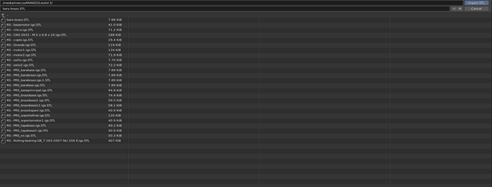
\includegraphics[scale=1.7]{3.png}
\caption{Archivos .STL}
\label{Imagen 4}
\end{figure}\\
Una vez abrimos el ensamble, observamos que nos faltan algunas piezas las cuales se colocan de manera manual por medio de la opción transformar y por medio de coordenadas, se colocan en el lugar deseado.
\begin{figure}[h]
	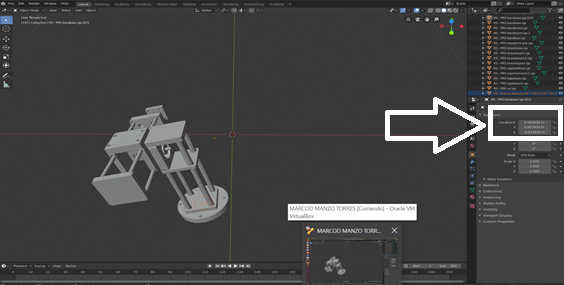
\includegraphics[scale=1.2]{4.png}
	\caption{Ensamble importado}
	\label{Imagen 4}
\end{figure}\\
Ahora que finalizamos el ensamble importado en Blender, guardamos el mismo como archivo .DAE y lo colocamos en nuestra carpeta launcher de Gazebo
\begin{figure}[h]
	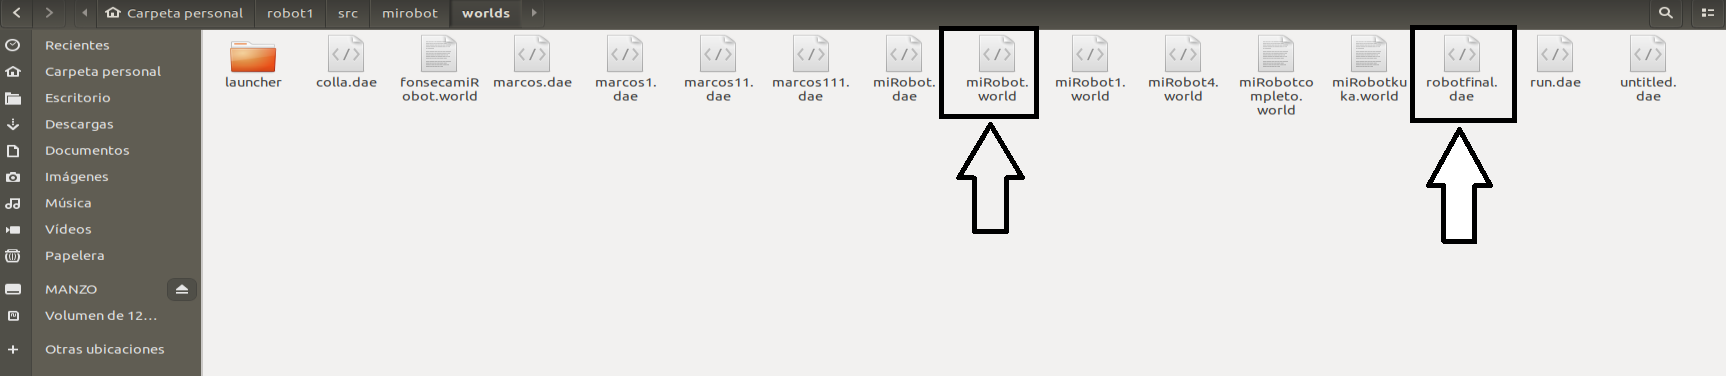
\includegraphics[scale=.5]{carpeta.png}
	\caption{Guardar ensamble}
	\label{Imagen 5}
\end{figure}\\
Observamos la información almacenada en nuestro archivo .DAE, donde nuestro ensamble fue guardado por medio de mallas similar a un archivo .USDF que es el archivo base de Gazebo.
Encontramos cómo se declara el entorno y las uniones para que estas aparescan a la hora de correr el mismo.
\begin{figure}[h]
	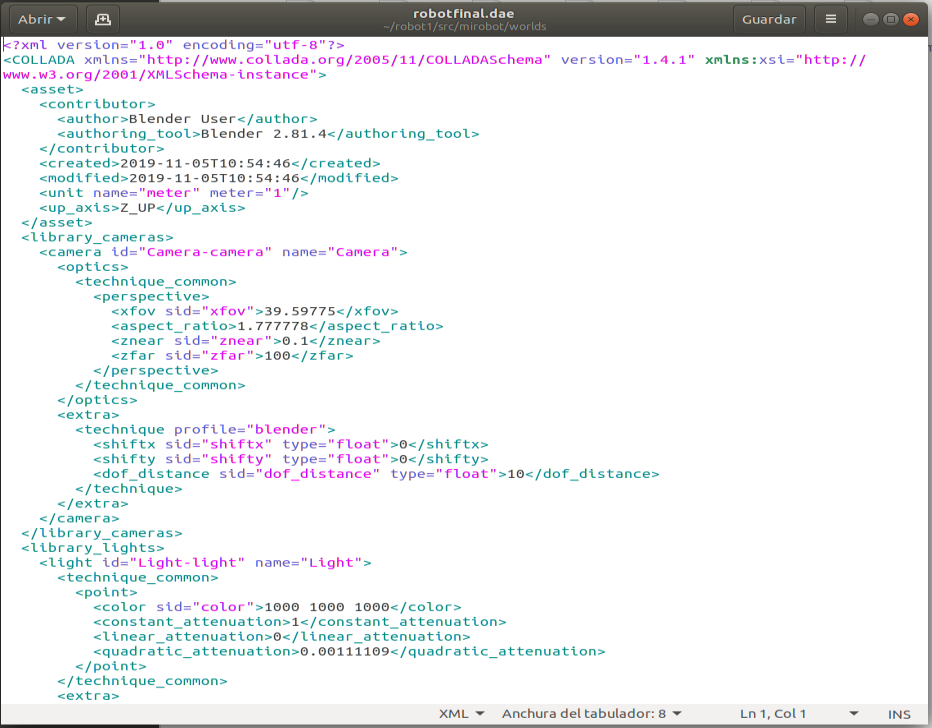
\includegraphics[scale=.45]{dae.png}
	\caption{Archivo .DAE}
	\label{Imagen 6}
\end{figure}\\
Para iniciar el contenido en Gazebo, necesitamos declarar un archivo .World el cual funciona como launcher para iniciar el contenido o arrancar el contenido especificado. solo basta con colocar el nombre del archivo .DAE que deseamos iniciar.
\begin{figure}[h]
	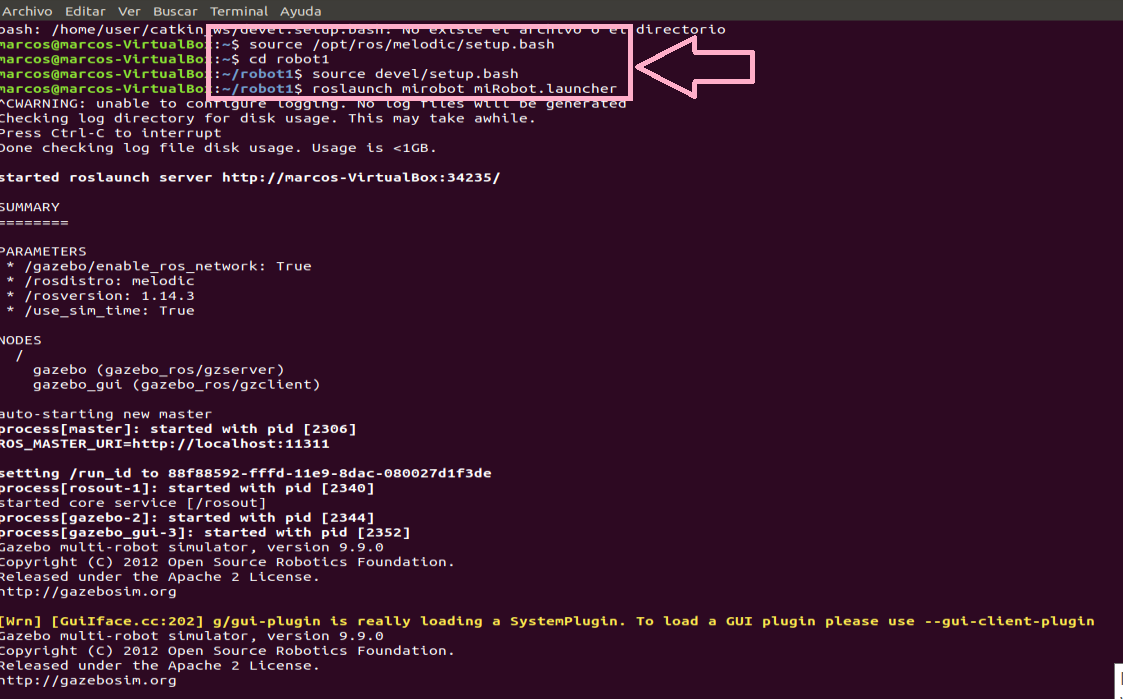
\includegraphics[scale=.45]{6.png}
	\caption{Arrancador}
	\label{Imagen 7}
\end{figure}
Ahora solo basta abrir un terminal, donde iniciaremos gazebo y nos abrirá nuestro archivo colocado en el arrancador y en nuestra carpeta de trabajo.
\begin{figure}[h]
	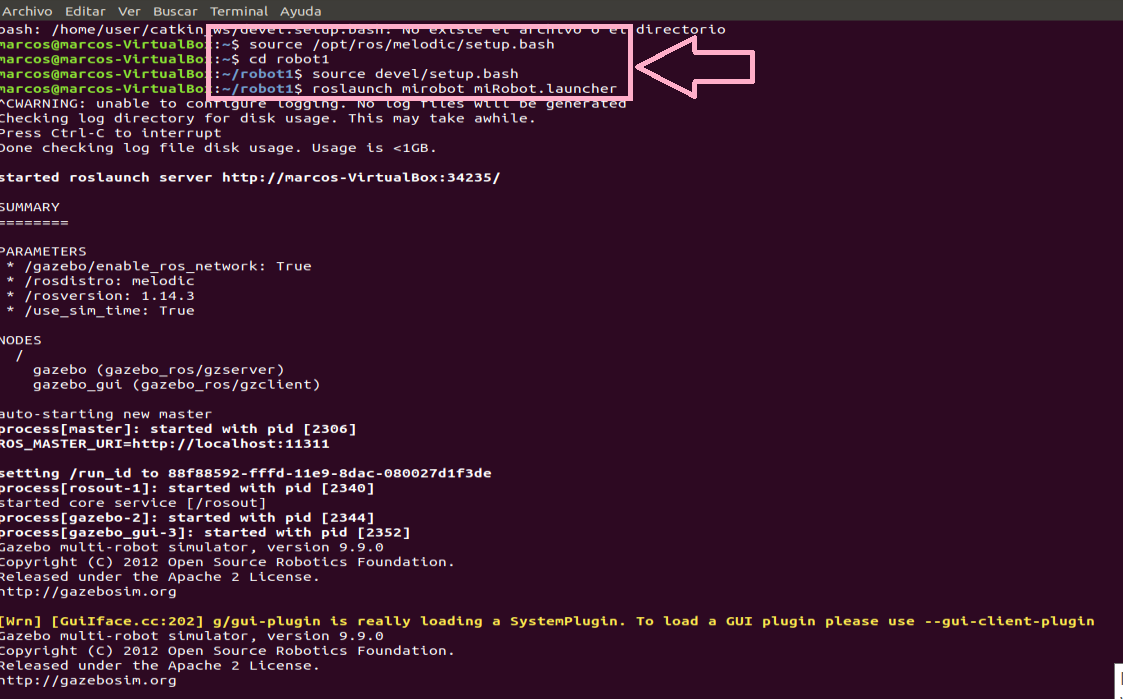
\includegraphics[scale=.75]{iniciargaz.png}
	\caption{Iniciar Gazebo}
	\label{Imagen 8}
\end{figure}\\
Tras haber iniciado Gazebo en nuestra terminal, podemos observar una ventana nueva donde nos aparece el contenido y su entorno, además de poder observar a detalle la simluación de nuestro robot.
\begin{figure}[h]
	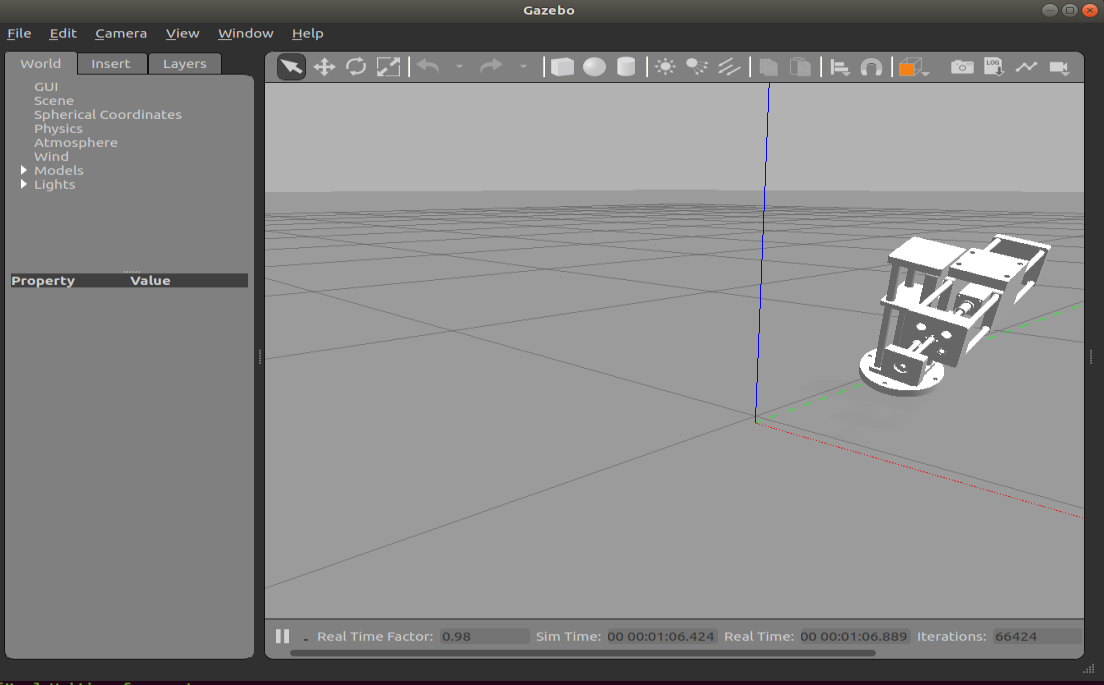
\includegraphics[scale=.75]{gaz.png}
	\caption{Gazebo}
	\label{Imagen 9}
\end{figure}
\chapter{conclusión}
Con esta práctica hemos aprendido a realizar el "traslado" de un modelado tridimensional no solo de un programa a otro, sino que también de un sistema operativo a otro.\\
Esta herramienta nos será de utilidad en prácticas posteriores, donde será necesario simular el funcionamiento de nuestro robot esférico polar de manera virtual y corroborar su correcto funcionamiento sin el temor de algún desastre en el modelo físico, esto de la mano con ROS, para posteriormente poder aplicar nuestra programación en el modelo físico final.


\hfill
\bibliographystyle{unsrt}
\bibliography{torres}


\end{document}

